\let\negmedspace\undefined
\let\negthickspace\undefined

\documentclass[journal,12pt,onecolumn]{IEEEtran}
%\documentclass[journal,12pt,twocolumn]{IEEEtran}
%
\usepackage{setspace}
\usepackage{gensymb}
%\doublespacing
\singlespacing

%\usepackage{graphicx}
%\usepackage{amssymb}
%\usepackage{relsize}
\usepackage[cmex10]{amsmath}
%\usepackage{amsthm}
%\interdisplaylinepenalty=2500
%\savesymbol{iint}
%\usepackage{txfonts}
%\restoresymbol{TXF}{iint}
%\usepackage{wasysym}
\usepackage{amsthm}
\usepackage{mathrsfs}
\usepackage{txfonts}
\usepackage{stfloats}
\usepackage{cite}
\usepackage{cases}
\usepackage{subfig}
%\usepackage{xtab}
\usepackage{longtable}
\usepackage{multirow}
%\usepackage{algorithm}
%\usepackage{algpseudocode}
\usepackage{enumitem}
\usepackage{mathtools}
\usepackage{tikz}
\usepackage{circuitikz}
\usepackage{verbatim}
\usepackage{hyperref}
%\usepackage{stmaryrd}
\usepackage{tkz-euclide} % loads  TikZ and tkz-base
%\usetkzobj{all}
\usepackage{listings}
\usepackage{color}                                            %%
\usepackage{array}                                            %%
\usepackage{longtable}                                        %%
\usepackage{calc}                                             %%
\usepackage{multirow}                                         %%
\usepackage{hhline}                                           %%
\usepackage{ifthen}                                           %%
%optionally (for landscape tables embedded in another document): %%
\usepackage{lscape}     
\usepackage{multicol}
\usepackage{chngcntr}
\usepackage{iftex}
%\usepackage[latin9]{inputenc}
\usepackage{geometry}
\usepackage{bm}
%\geometry{verbose,tmargin=2cm,bmargin=3cm,lmargin=1.8cm,rmargin=1.5cm,headheight=2cm,headsep=2cm,footskip=3cm}
\usepackage{array}
\newcolumntype{L}[1]{>{\raggedright\let\newline\\\arraybackslash\hspace{0pt}}m{#1}}
\newcolumntype{C}[1]{>{\centering\let\newline\\\arraybackslash\hspace{0pt}}m{#1}}
\newcolumntype{R}[1]{>{\raggedleft\let\newline\\\arraybackslash\hspace{0pt}}m{#1}}

%\usepackage{graphicx}
%\usepackage{setspace}
%\usepackage{parskip}

\def \hsp {\hspace{3mm}}

\makeatletter

\providecommand{\tabularnewline}{\\}



\makeatother
\ifxetex
\usepackage[T1]{fontenc}
\usepackage{fontspec}
%\setmainfont[ Path = fonts/]{Sanskrit_2003.ttf}
\newfontfamily\nakulafont[Script=Devanagari,AutoFakeBold=2,Path = fonts/]{Nakula}
%\newfontfamily\liberationfont{Liberation Sans Narrow}
%\newfontfamily\liberationsansfont{Liberation Sans}
\fi
\usepackage{tikz}
\usepackage{xcolor}
%\usepackage{enumerate}

%\usepackage{wasysym}
%\newcounter{MYtempeqncnt}
\DeclareMathOperator*{\Res}{Res}
%\renewcommand{\baselinestretch}{2}
\renewcommand\thesection{\arabic{section}}
\renewcommand\thesubsection{\thesection.\arabic{subsection}}
\renewcommand\thesubsubsection{\thesubsection.\arabic{subsubsection}}

\renewcommand\thesectiondis{\arabic{section}}
\renewcommand\thesubsectiondis{\thesectiondis.\arabic{subsection}}
\renewcommand\thesubsubsectiondis{\thesubsectiondis.\arabic{subsubsection}}

% correct bad hyphenation here
\hyphenation{op-tical net-works semi-conduc-tor}
\def\inputGnumericTable{}                                 %%

\lstset{
	language=tex,
	frame=single, 
	breaklines=true
}

%\begin{document}
%


\newtheorem{theorem}{Theorem}[section]
\newtheorem{problem}{Problem}
\newtheorem{proposition}{Proposition}[section]
\newtheorem{lemma}{Lemma}[section]
\newtheorem{corollary}[theorem]{Corollary}
\newtheorem{example}{Example}[section]
\newtheorem{definition}[problem]{Definition}
%\newtheorem{thm}{Theorem}[section] 
%\newtheorem{defn}[thm]{Definition}
%\newtheorem{algorithm}{Algorithm}[section]
%\newtheorem{cor}{Corollary}
\newcommand{\BEQA}{\begin{eqnarray}}
	\newcommand{\EEQA}{\end{eqnarray}}
\newcommand{\define}{\stackrel{\triangle}{=}}
\bibliographystyle{IEEEtran}
%\bibliographystyle{ieeetr}
\providecommand{\mbf}{\mathbf}
\providecommand{\pr}[1]{\ensuremath{\Pr\left(#1\right)}}
\providecommand{\qfunc}[1]{\ensuremath{Q\left(#1\right)}}
\providecommand{\sbrak}[1]{\ensuremath{{}\left[#1\right]}}
\providecommand{\lsbrak}[1]{\ensuremath{{}\left[#1\right.}}
\providecommand{\rsbrak}[1]{\ensuremath{{}\left.#1\right]}}
\providecommand{\brak}[1]{\ensuremath{\left(#1\right)}}
\providecommand{\lbrak}[1]{\ensuremath{\left(#1\right.}}
\providecommand{\rbrak}[1]{\ensuremath{\left.#1\right)}}
\providecommand{\cbrak}[1]{\ensuremath{\left\{#1\right\}}}
\providecommand{\lcbrak}[1]{\ensuremath{\left\{#1\right.}}
\providecommand{\rcbrak}[1]{\ensuremath{\left.#1\right\}}}
\theoremstyle{remark}
\newtheorem{rem}{Remark}
\newcommand{\sgn}{\mathop{\mathrm{sgn}}}
\providecommand{\abs}[1]{\left\vert#1\right\vert}
\providecommand{\res}[1]{\Res\displaylimits_{#1}} 
\providecommand{\norm}[1]{\left\lVert#1\right\rVert}
%\providecommand{\norm}[1]{\lVert#1\rVert}
\providecommand{\mtx}[1]{\mathbf{#1}}
\providecommand{\mean}[1]{E\left[ #1 \right]}
\providecommand{\fourier}{\overset{\mathcal{F}}{ \rightleftharpoons}}
%\providecommand{\hilbert}{\overset{\mathcal{H}}{ \rightleftharpoons}}
%\providecommand{\system}{\overset{\mathcal{H}}{ \longleftrightarrow}}
\providecommand{\system}[1]{\overset{\mathcal{#1}}{ \longleftrightarrow}}
\providecommand{\gauss}[2]{\mathcal{N}\ensuremath{\left(#1,#2\right)}}
%
%\newcommand{\solution}[2]{\textbf{Solution:}{#1}}
\newcommand{\solution}{\noindent \textbf{Solution: }}
\newcommand{\cosec}{\,\text{cosec}\,}
\newcommand{\sinc}{\,\text{sinc}\,}
\newcommand{\rect}{\,\text{rect}\,}
\providecommand{\dec}[2]{\ensuremath{\overset{#1}{\underset{#2}{\gtrless}}}}
\newcommand{\myvec}[1]{\ensuremath{\begin{pmatrix}#1\end{pmatrix}}}
\newcommand{\mydet}[1]{\ensuremath{\begin{vmatrix}#1\end{vmatrix}}}
\newcommand*{\permcomb}[4][0mu]{{{}^{#3}\mkern#1#2_{#4}}}
\newcommand*{\perm}[1][-3mu]{\permcomb[#1]{P}}
\newcommand*{\comb}[1][-1mu]{\permcomb[#1]{C}}
%\numberwithin{equation}{section}
\numberwithin{equation}{section}
%\numberwithin{problem}{section}
%\numberwithin{definition}{section}
\makeatletter
\@addtoreset{figure}{problem}
\makeatother
%\let\StandardTheFigure\thefigure
\let\vec\mathbf
%\renewcommand{\thefigure}{\theproblem.\arabic{figure}}
\renewcommand{\thefigure}{\arabic{section}.\arabic{figure}}
%\setlist[enumerate,1]{before=\renewcommand\theequation{\theenumi.\arabic{equation}}
	%\counterwithin{equation}{enumi}
	%\renewcommand{\theequation}{\arabic{subsection}.\arabic{equation}}
\let\StandardTheFigure\thefigure
	\vspace{3cm}
	%\usepackage{babel}
	\begin{document}
	 \title{Support Vector Machines}
	 \author{Mannem Charan AI21BTECH11019}
	 \maketitle
	   \begin{abstract}
		This report consists of my basic understanding of one of the popular Ml methods "Support Vector Machines".
	   \end{abstract}
           \section{Support Vector Machines}
	     SVM, Support Vector Machines is a supervised learning model which is used to solve classification and regression problems.Though we say regression, it is predominantly used for classification problems.SVM in general is used to find a decision boundary known as "\textbf{hyperplane}" to  classify the data.And the dimensions of hyper plane depends on features/predictors of the data point.It is used for binary classification and in case of multi class it breaks the problem into multiple binary classification problems.
	   \section{Types of SVM}
	     Based on the dataset given, SVM are of two types,
	      \begin{enumerate}
		      \item \textbf{Linear SVM}:We use linear SVM when the data is \textbf{"linearly Seperable"}, when we say linearly seperable we mean that we that one can find a line(if\, one\, line\, exists\, then\, \textbf{infinitely}\, many\, lines\, are\, possible) which can classify the data into two classes.\\
		       Ex: Hard-margin SVM
                      \item \textbf{Non-linear SVM}:We use Non-linear SVM when the data is not linearly seperable i.e., we can't find a straight line which can classify the data into two classes.\\
		       Ex: Soft-margin classifier, kernals
	      \end{enumerate}
	    \section{Linear SVM}
	      If the data is linearly seperable,then we can find infinitely many lines/hyperplanes to classify the data but some may lead to the chance of overfitting.So we choose a hyperplane which can classify the given data and have less generalisation error.To do that, we take the help of some data points known as "Support Vectors",the data points(of\,either\,class) which are close to the hyperplane.And the gap between these data points and the hyperplane is known as "Margin".So we use these support vectors to adjust the hyperplane by maximising the margin(in \, case \, of\, linear\, SVM).Since these vectors supporting the hyperplane, they are known as "Support Vectors".That's why the algorithm is named after them as "Support Vector Machines".First it is introduced as Support Vector Networks but then machine word became popular and people started using it as SVM.
	    \section{Understanding Linear SVM}
	    As we said earlier, we use Linear SVM when we have linearly seperable data.Let us define the labelled data as $\cbrak{\brak{\vec{x_1},y_1},\,.\,.\,.\brak{\vec{x_k},y_k}}$ where ,
	       \begin{enumerate}
	         \item k = no. of features
	         \item $x_i$ = $i^{th}$ data point
		 \item $y_i$ = label of $x_i$ and $y_i \in \cbrak{-1,1}$
	       \end{enumerate}
	 Mathematically, to say that the dataset is linearly seperable, we should be able to find a $\brak{\vec{w},\theta}$ such that,
	       \begin{align}
		      \vec{w}^T\vec{x} - \theta &= \begin{cases}
			                               \geq 0 &,y_i = 1\\
						        < 0   &, y_i = -1
					           \end{cases} 
	       \end{align}
	    The above expression follows from the fact that the hyperplane classifies the data correctly.So one can find infinetly many $\vec{w}$ and $\theta$ that can satisfy above expression.So one of the classical methods to choose the optimal hyper plane is to \textbf{maximise} the margin.First, to find the margin we will draw parralel lines to the hyperplane that are passing through the support vectors.As you can see in the figure $\ref{Fig 1}$,\\
	       \begin{figure}[h]
		\centering
		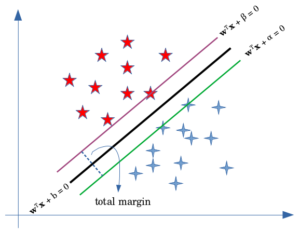
\includegraphics[width = 10cm]{margin.png}
		\caption{Linearly seperable data}
		\label{Fig 1}
	       \end{figure}
	    let say the two parallel hyperplanes are
	       \begin{align}
		       \vec{w}^T\vec{x} + \alpha &= 0\\
		       \vec{w}^T\vec{x} + \beta &= 0
               \end{align}
	     And in this case let say $\vec{w}^T\vec{x} + b = 0$ be the hyperplane.So since we want to maximise the margin,we should maximise the distance between the two hyperplanes i.e, we want to maximise
	       \begin{align}
		       d = \frac{\abs{\alpha - \beta}}{\norm{w}}
	       \end{align}
	       So to the maximise the margin $\frac{\abs{\alpha - \beta}}{\norm{w}}$, we should minimise the norm $\norm{w}$. Now to make things simple let us take $\alpha = b + 1$ and $\beta = b - 1$, now the constraints will be 
	        \begin{align}
			\vec{w}^T\vec{x} - \theta &= \begin{cases} \label{constraints}
                                                       \geq 1 &,y_i = 1\\
                                                        < -1   &, y_i = -1
                                                   \end{cases} 
                \end{align} 
		So the same thing can be written as ,
		\begin{align}
			y_i\brak{\vec{w}^T\vec{x} - \theta} \geq 1
		\end{align}
		Because we want to classify the data point to class $+1$ whenever $\vec{w}^T\vec{x} + b \geq 1$ and to class $-1$ whenever $\vec{w}^T\vec{x} + b < -1$.So the margin in this case is $\frac{2}{\norm{w}}$ and to maximise it we should minimise,
		\begin{align}
		    \frac{\norm{w}}{2}
	        \end{align}
		Now to make math simple we will try to minimise,
		\begin{align}
			\frac{\norm{w}^2}{2} &= \frac{1}{2}\vec{w}^T\vec{w}
	        \end{align}
 So here the cost function will be 
                \begin{align}
			J &= \frac{1}{2}\vec{w}^T\vec{w}
		\end{align}
		with the constraints mentioned in $\eqref{constraints}$.By minimising the cost function we will find the optimal hyperplane needed.\\
	This method is also known as "Hard - margin" SVM since we are strictly classifying the data points using the margin.But often we don't have linearly seperable data in those cases we either relax the margin or use some kernel tricks.
	  \section{Understanding Non-linear SVM}
	    When we can't divide the data using a straight line, we generally follow two approaches,
	         \begin{enumerate}
		   \item \textbf{Soft -margin}: Where we try to relax the margin to allow some data points to misclassify.
	           \item \textbf{Kernal besed approach}: In this case, we try to transform the training data(low\, dimensional\, data) into a high dimesional space in order to make the data linearly seperable.
	         \end{enumerate}
            \section{Soft-Margin}
	      When the data is not linearly seperable then maximising the margin is not a suitable method,in that case we try to relax the margin and allow some data points to misclassify.To do that we will add some new variables known as "Slack variables". These variables try to relax the margin and allow some points to misclassify.So the new constraints will be,
	           \begin{align}
			   y_i\brak{\vec{w}^T\vec{x} -\theta} \geq 1-\xi_i \brak{i = 0,\,1,\,.\,.\,.,\,k}\label{constraints1}
                   \end{align}
And if $0\leq \xi_i \leq 1$ then the inner product stil have the same sign but with a reduced margin but if $\xi_i > 1$ then that data point will be misclassified.\\
Since we are allowing the data points to misclassify, we should minimise the error as low as possible.We call this error as "Hinge loss" and this is nothing but the lossoccured to a misclassified point i.e., $\xi_i$.That's why the cost function for soft-margin classifier is,
                   \begin{align}
			   \norm{\vec{w}}^2 + C\sum_{i=1}^k\xi_i
                   \end{align}
		with the constraints mentioned in $\eqref{constraints1}$.And constant C is a tuning parameter which helps in adjusting the count of how many points to be misclassifed.If $C =0$, then model reverts back to hard-margin classifier.And as C increases the violation of data points increases.Therefore soft-margin classifier can be considered as a more generalised form of Hard-margin classifier.You can visualise the same in Fig $\ref{Fig 2}$.\\
		 \begin{figure}[!h]
	          \centering
		  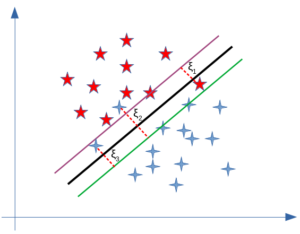
\includegraphics[width = 10cm]{soft-margin.png}
		  \caption{A soft-margin classifier allows the data points\brak{\text{can\, be\, outliers}} to misclassify in order to generalise better}
	          \label{Fig 2}
	         \end{figure}
 		And moreover even though data is linearly seperable if the margin is too low,then the model have a risk of overfitting or it may become sensitive to the outliers.Hence in that case we can opt for a large margin by choosing soft-margin SVM in order to help the model generalise better.
            \section{Kernal Based Approach}
	     In SVM, to deal with non-linear data although we have soft-margin SVM we will try use some techniques known as kernel tricks which actually classifies the given data in the higher dimensional space.First we try to map our feature set to an enlarged feature set,to understand that let us see an example Fig $\ref{Fig 3}$\\
	         \begin{figure}
	           \centering
	           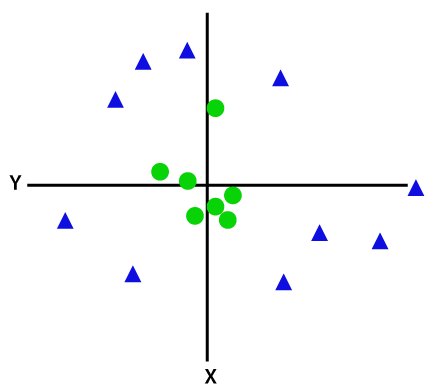
\includegraphics[width =5cm]{kernal.png}
	           \caption{Non -linear data}
		   \label{Fig 3}
	         \end{figure}
     The Fig $\ref{Fig 3}$ represents a dataset with two features $x$ and $y$. And you can see, the data is not linearly seperable so it try to add a new dimension to the feature set let say $z$ which depends on $x$ and $y$ as follows,
                 \begin{align}
			z = x^2 + y^2
	         \end{align}
		 So the new data looks like Fig $\ref{Fig 4}$,
		  \begin{figure}
		   \centering
		   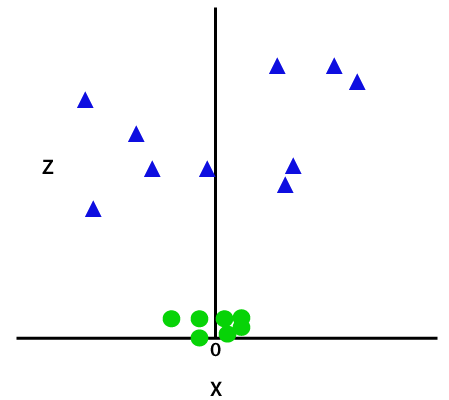
\includegraphics[width = 5cm]{kernal2.png}
		   \caption{Linear data after transforamation}
		   \label{Fig 4}
		  \end{figure}
	  and since it is linearly seperable we can find the suitable hyperplane to classify this new data.Since the data has 3 dimensions the hyperplane will be of 2 dimensions i.e., a plane.
            So when we see it from above the data will appeared to be classified with a curve as shown in fig $\ref{Fig 5}$.
	          \begin{figure}
		       \centering
	           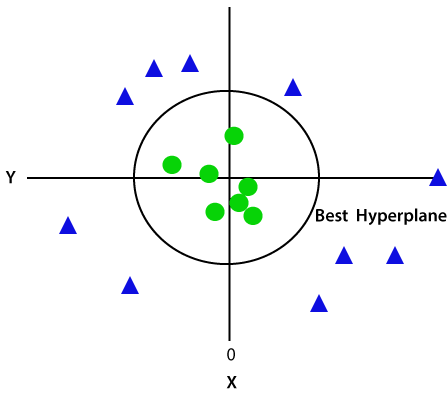
\includegraphics[width= 5cm]{kernal3.png}
	           \caption{Data is classified with a circle}
		       \label{Fig 5}
		  \end{figure}
      So as we saw in this example,in general we try to map the given feature dataset to a enlarged dataset and then classify it using our knowledge of linear SVM.
             \section{Questions}
              \begin{enumerate}
	        \item What is a hyperplane?
	        \item What are support vectors in SVM?
	        \item What is the difference between hard-margin and soft-margin SVM?
		\item What is the role of $C$ in soft-margin SVM?
		\item What is a kernel trick?
	      \end{enumerate}
	     \section{Solutions}
	       \begin{enumerate}
	         \item Hyperplane is a decision boundary used to classify the data into two classes. The dimensions of the hyper plane depends of the feature set of the dataset and it is 1 less than the dimensions of features.
	         \item Support vectors are the data points(of\, either\, class) which are close to the hyper plane.And these support vectors help in building the hyper plane.
	         \item 
		      \begin{itemize}
			\item Hard-margin SVM is used for linear data whereas soft-margin SVM is used for non-linear data
		        \item In soft-margin we will allow some points to misclassify whereas in hard-margin, we will try classify the data correctly.
		        \item Soft-margin generalises better in case of outliers whereas the performance of hard-margin depends on the position of outlier(whether\, there\, are\, close\, to\, hyperplane\, or\, not)
		      \end{itemize}
	          \item The $C$ is the tuning parameter for the soft-margin model, where
			   \begin{itemize}
			     \item The smaller the value of $C$, the more sensitive the algorithm is to the training data.
			     \item The larger the value of $C$, the less sensitive the algorithm is to the training data.
		           \end{itemize}
	          \item The kernel technique is a method to transform a non-linear data into a higher dimensional space to make the data suitable for classification.It involves adding new features using the orginal feature set.
	        \end{enumerate}
      \end{document}	      











